% Exemplo de dissertação do INF-UFG com texto em portugues formatado com LaTeX
\documentclass[tese, abnt]{inf-ufg}
% Opções da classe inf-ufg (ao usar mais de uma, separe por vírgulas)
%   [tese]         -> Tese de doutorado.
%   [dissertacao]  -> Dissertação de mestrado (padrão).
%   [monografia]   -> Monografia de especialização.
%   [relatorio]    -> Relatório final de graduação.
%   [abnt]         -> Usa o estilo "abnt-alf" de citação bibliográfica.
%   [nocolorlinks] -> Os links de navegação no texto ficam na cor preta.
%                     Use esta opção para gerar o arquivo para impressão
%                     da versão final do seu texto!!!
%% Colocado Autor

\usepackage[utf8]{inputenc}

\usepackage[T1]{fontenc}
\usepackage[normalem]{ulem} % riscos no texto
\usepackage{graphicx}
\usepackage{import}
\usepackage{xspace}

%% fim colocado autor

%----------------------------------------------------- INICIO DO DOCUMENTO %
\begin{document}

%------------------------------------------ AUTOR, TÍTULO E DATA DE DEFESA %
\autor{Seu nome}
\autorR{Sobrenome, Nome}

\titulo{Titulo}
%\subtitulo{}

\cidade{Goiânia}
\dia{02}
\mes{07}
\ano{2019} % Formato numérico: \dia{01}, \mes{01} e \ano{2009}

%-------------------------------------------------------------- ORIENTADOR %
\orientador{Orientador}
\orientadorR{Sobrenome, Nome}
% Use os comandos a seguir se for Orientadora e nao Orientador.
%\orientadora{\textless Nome da Orientadora\textgreater}
%\orientadoraR{\textless Nome Reverso da Orientadora\textgreater}

%\coorientador{\textless Nome do Co-orientador\textgreater}
%\coorientadorR{\textless Nome Reverso do Co-orientador\textgreater}
% Use os comandos a seguir se for Co-orientadora e nao Coorientador.
%\coorientadora{\textless Nome da Co-orientadora\textgreater}
%\coorientadoraR{\textless Nome Reverso da Co-orientadora\textgreater}

%-------------------------------------------------- INSTITUIÇÃO E PROGRAMA %
\universidade{Universidade Federal de Goiás}
\uni{UFG}
\unidade{Instituto de Informática}
\departamento{} % Unidades com mais de um departamento.

%\universidadeco{\textless Nome da Universidade do Co-orientador\textgreater}
%\unico{\textless Sigla da Universidade do Co-orientador\textgreater}
%\unidadeco{\textless Nome da Unidade Acadêmica do Co-orientador\textgreater}

\programa{Ciência da Computação}
\concentracao{Ciência da Computação}

%-------------------------------------------------- ELEMENTOS PRÉ-TEXTUAIS %
\capa    % Gera o modelo da capa externa do trabalho
%\publica % Gera a autorização para publicação em formato eletrônico
\rosto   % Primeira folha interna do trabalho

%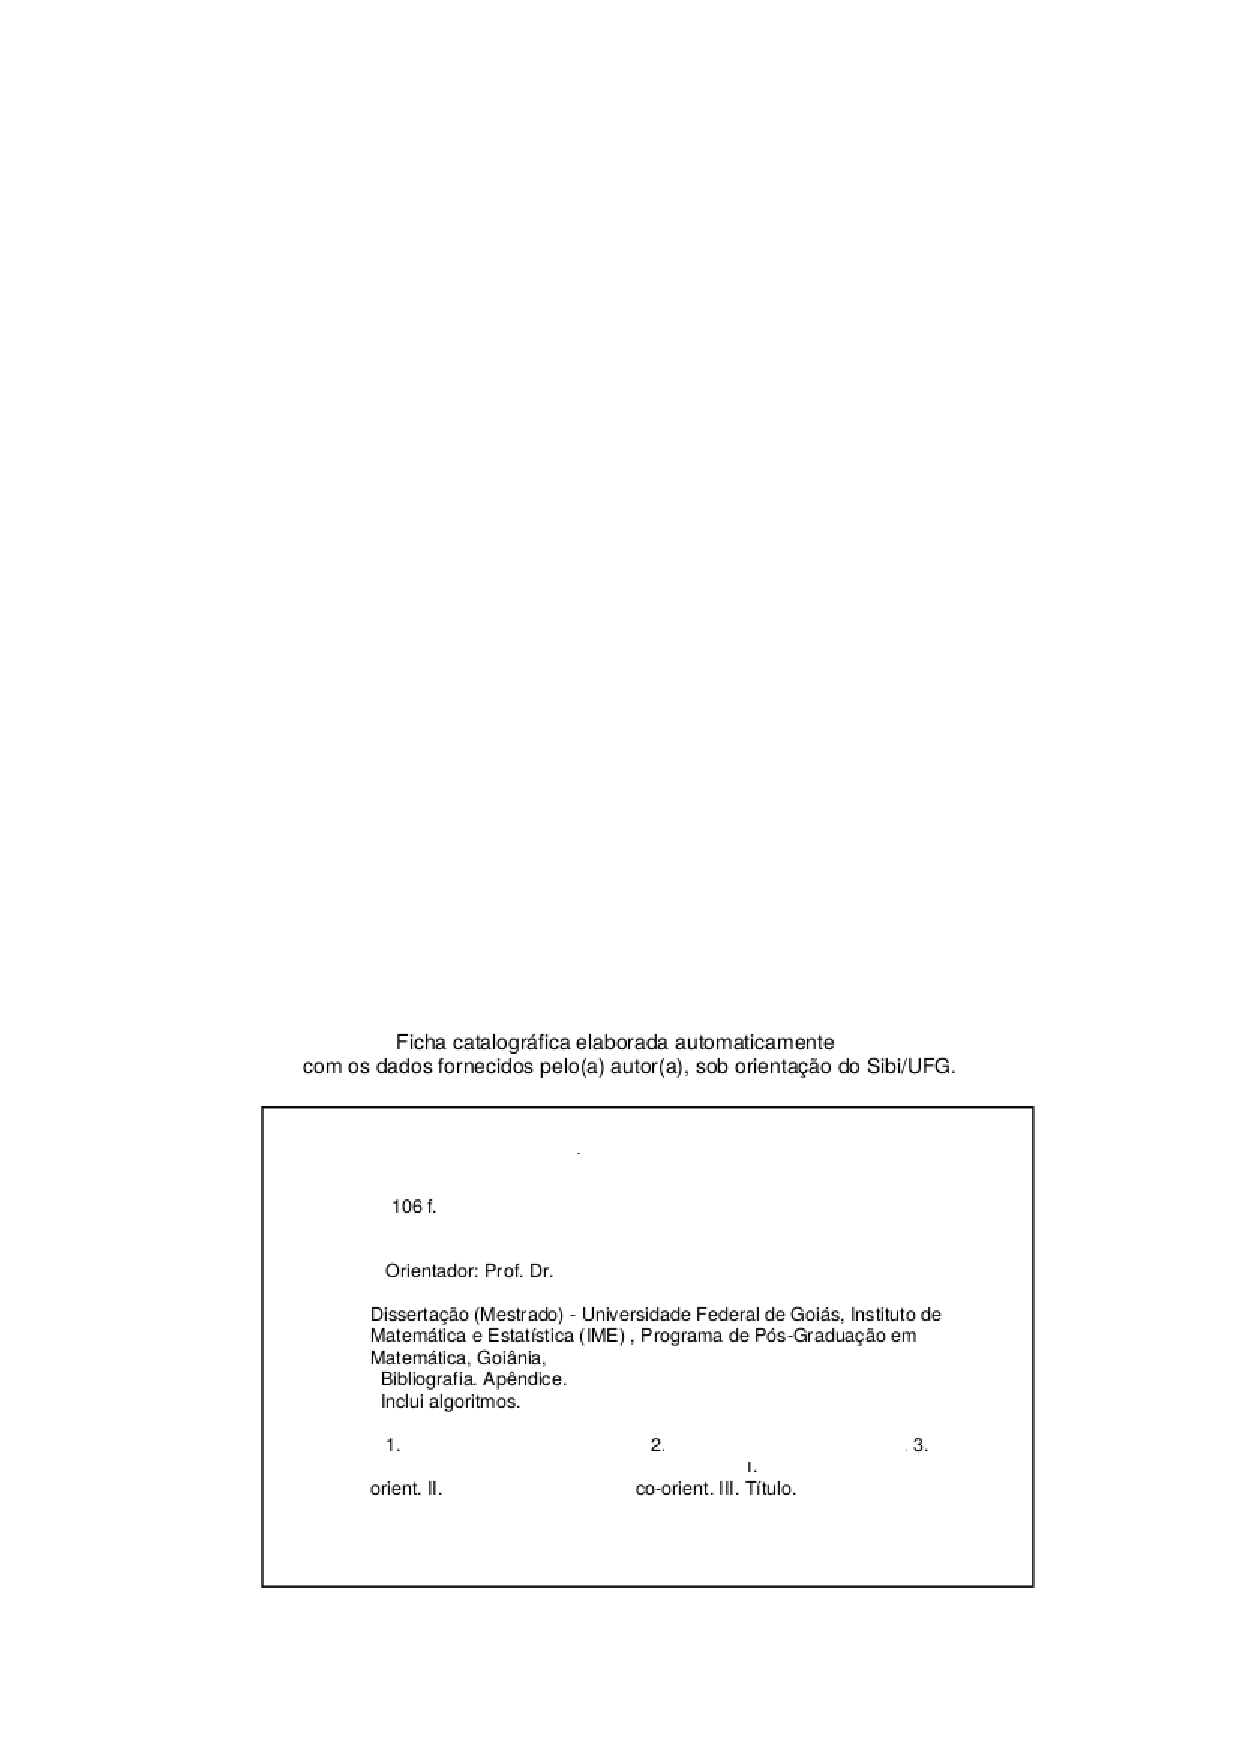
\includepdf[pages={1},templatesize={250mm}{297mm}]{./pre/FichaCatalografica.pdf}  %Ficha Catalográfica expedida pela secretaria do programa
%\begin{aprovacao}
\banca{Dr. Membro da Banca 1}{Instituto de Informática\ -- UFG}
\banca{Dr. Membro da Banca 2}{Instituto de Informática\ -- UFG}
% Use o comando \profa se o membro da banca for do sexo feminino.
\banca{Dr. Membro Externo}{Faculdade de Fora\ -- FF}
\end{aprovacao}
%\direitos{\textless Texto com um perfil resumido do autor do trabalho. Por exemplo: (Graduou--se em Artes Cênicas na UFG - Universidade Federal de Goiás. Durante sua graduação, foi monitor no departamento de Filosofia da UFG e pesquisador do CNPq em um trabalho de iniciação científica no departamento de Biologia. Durante o Mestrado, na USP - Universidade de São Paulo, foi bolsista da FAPESP e desenvolveu um trabalho teórico na resolução do Problema das Torres de Hanói. Atualmente desenvolve soluções para problemas de balanceamento de ração para a pecuária de corte.)\textgreater}


%\begin{dedicatoria}
\textless Dedicatória do trabalho a alguma pessoa, entidade, etc.\textgreater
\end{dedicatoria}
%\begin{agradecimentos}
\textless Texto com agradecimentos àquelas pessoas/entidades que, na opinião do autor, deram alguma contribuíção relevante para o desenvolvimento do trabalho.\textgreater
\end{agradecimentos}



%\epigrafe{\textless Epígrafe é uma citação relacionada com o tópico do texto\textgreater}
{\textless Nome do autor da citação\textgreater}
{\textless Título da referência à qual a citação pertence\textgreater}

\chaves{Palavra 1, Palavra 2, Palavra 3, Palavra 4}

\begin{resumo} 

\end{resumo}


\keys{key 1, Key 2, key 3, key 4}

\begin{abstract}{titulo}

\end{abstract}


\begin{ListaSiglas}

\begin{siglas}
  \item \textbf{[WEKA]} Suite de Ferramentas de Mineração de Dados
  \item \textbf{[WEKA]} Suite de Ferramentas de Mineração de Dados
  \item \textbf{[WEKA]} Suite de Ferramentas de Mineração de Dados
  \item \textbf{[WEKA]} Suite de Ferramentas de Mineração de Dados
  \item \textbf{[WEKA]} Suite de Ferramentas de Mineração de Dados
  \item \textbf{[WEKA]} Suite de Ferramentas de Mineração de Dados
\end{siglas}

\end{ListaSiglas}




\tabelas[figtabalg]
%\textcolor{red}{texto}
%\tabelas[figtabalgcod]
%Opções:
%nada [] -> Gera apenas o sumário
%fig     -> Gera o sumário e a lista de figuras
%tab     -> Sumário e lista de tabelas
%alg     -> Sumário e lista de algoritmos
%cod     -> Sumário e lista de códigos de programas
%
% Pode-se usar qualquer combinação dessas opções.
% Por exemplo:
%  figtab       -> Sumário e listas de figuras e tabelas
%  figtabcod    -> Sumário e listas de figuras, tabelas e
%                  códigos de programas
%  figtabalg    -> Sumário e listas de figuras, tabelas e algoritmos
%  figtabalgcod -> Sumário e listas de figuras, tabelas, algoritmos e
%                  códigos de programas

%Lista de Siglas



%--------------------------------------------------------------- CAPÍTULOS %
%\import{sections/}{section1.tex}
\chapter{Introdução}
\label{cap:01}




\chapter{Contexto e Descrição do Problema}
\label{cap:02}




 
\chapter{Proposta}
\label{cap:03}






\chapter{Resultados}
\label{cap:04}







\chapter{Conclusão}
\label{cap:05}



%------------------------------------------------------------ BIBLIOGRAFIA %
%\cleardoublepag e
%\nocite{*} %%% Retire esta linha para gerar a bibliografia com apenas as
           %%% referências usadas no seu texto!
\arial
\bibliography{/bib/bibliografia} %%% Nomes dos seus arquivos .bib
\label{ref-bib}

%--------------------------------------------------------------- APÊNDICES %
\apendices

%\chapter{Exemplo de um Apêndice}
\label{apend:1}
$ \alpha, \beta, \ldots, \omega $ \newline
Apêndicess são iniciados com o comando \verb|\apendices|.
Apêndicess são iniciados com o comando \verb|\apendices|.
Apêndicess são iniciados com o comando \verb|\apendices|.
Apêndicess são iniciados com o comando \verb|\apendices|.
Apêndicess são iniciados com o comando \verb|\apendices|.
Apêndicess são iniciados com o comando \verb|\apendices|.
Apêndicess são iniciados com o comando \verb|\apendices|.
Apêndicess são iniciados com o comando \verb|\apendices|.
Apêndicess são iniciados com o comando \verb|\apendices|.
Apêndicess são iniciados com o comando \verb|\apendices|.
Apêndicess são iniciados com o comando \verb|\apendices|.
Apêndicess são iniciados com o comando \verb|\apendices|.
Apêndicess são iniciados com o comando \verb|\apendices|.
Apêndicess são iniciados com o comando \verb|\apendices|.
Apêndicess são iniciados com o comando \verb|\apendices|.
Apêndicess são iniciados com o comando \verb|\apendices|.

Apêndicess são iniciados com o comando \verb|\apendices|.
Apêndicess são iniciados com o comando \verb|\apendices|.
Apêndicess são iniciados com o comando \verb|\apendices|.
Apêndicess são iniciados com o comando \verb|\apendices|.
Apêndicess são iniciados com o comando \verb|\apendices|.
Apêndicess são iniciados com o comando \verb|\apendices|.
Apêndicess são iniciados com o comando \verb|\apendices|.
Apêndicess são iniciados com o comando \verb|\apendices|.
Apêndicess são iniciados com o comando \verb|\apendices|.
Apêndicess são iniciados com o comando \verb|\apendices|.
Apêndicess são iniciados com o comando \verb|\apendices|.
Apêndicess são iniciados com o comando \verb|\apendices|.

Apêndicess são iniciados com o comando \verb|\apendices|.
Apêndicess são iniciados com o comando \verb|\apendices|.
Apêndicess são iniciados com o comando \verb|\apendices|.
Apêndicess são iniciados com o comando \verb|\apendices|.
Apêndicess são iniciados com o comando \verb|\apendices|.
Apêndicess são iniciados com o comando \verb|\apendices|.
Apêndicess são iniciados com o comando \verb|\apendices|.
Apêndicess são iniciados com o comando \verb|\apendices|.
Apêndicess são iniciados com o comando \verb|\apendices|.
Apêndicess são iniciados com o comando \verb|\apendices|.
Apêndicess são iniciados com o comando \verb|\apendices|.
Apêndicess são iniciados com o comando \verb|\apendices|.
Apêndicess são iniciados com o comando \verb|\apendices|.
Apêndicess são iniciados com o comando \verb|\apendices|.

Apêndicess são iniciados com o comando \verb|\apendices|.
Apêndicess são iniciados com o comando \verb|\apendices|.
Apêndicess são iniciados com o comando \verb|\apendices|.
Apêndicess são iniciados com o comando \verb|\apendices|.
Apêndicess são iniciados com o comando \verb|\apendices|.
Apêndicess são iniciados com o comando \verb|\apendices|.
Apêndicess são iniciados com o comando \verb|\apendices|.
Apêndicess são iniciados com o comando \verb|\apendices|.
Apêndicess são iniciados com o comando \verb|\apendices|.
Apêndicess são iniciados com o comando \verb|\apendices|.
Apêndicess são iniciados com o comando \verb|\apendices|.
Apêndicess são iniciados com o comando \verb|\apendices|.
Apêndicess são iniciados com o comando \verb|\apendices|.
Apêndicess são iniciados com o comando \verb|\apendices|.

Apêndicess são iniciados com o comando \verb|\apendices|.
Apêndicess são iniciados com o comando \verb|\apendices|.
Apêndicess são iniciados com o comando \verb|\apendices|.
Apêndicess são iniciados com o comando \verb|\apendices|.
Apêndicess são iniciados com o comando \verb|\apendices|.
Apêndicess são iniciados com o comando \verb|\apendices|.
Apêndicess são iniciados com o comando \verb|\apendices|.
Apêndicess são iniciados com o comando \verb|\apendices|.
Apêndicess são iniciados com o comando \verb|\apendices|.
Apêndicess são iniciados com o comando \verb|\apendices|.
Apêndicess são iniciados com o comando \verb|\apendices|.
Apêndicess são iniciados com o comando \verb|\apendices|.
Apêndicess são iniciados com o comando \verb|\apendices|.
Apêndicess são iniciados com o comando \verb|\apendices|.

Apêndicess são iniciados com o comando \verb|\apendices|.
Apêndicess são iniciados com o comando \verb|\apendices|.
Apêndicess são iniciados com o comando \verb|\apendices|.
Apêndicess são iniciados com o comando \verb|\apendices|.
Apêndicess são iniciados com o comando \verb|\apendices|.
Apêndicess são iniciados com o comando \verb|\apendices|.
Apêndicess são iniciados com o comando \verb|\apendices|.
Apêndicess são iniciados com o comando \verb|\apendices|.
Apêndicess são iniciados com o comando \verb|\apendices|.
Apêndicess são iniciados com o comando \verb|\apendices|.
Apêndicess são iniciados com o comando \verb|\apendices|.
Apêndicess são iniciados com o comando \verb|\apendices|.
Apêndicess são iniciados com o comando \verb|\apendices|.
Apêndicess são iniciados com o comando \verb|\apendices|.

Apêndicess são iniciados com o comando \verb|\apendices|.
Apêndicess são iniciados com o comando \verb|\apendices|.
Apêndicess são iniciados com o comando \verb|\apendices|.
Apêndicess são iniciados com o comando \verb|\apendices|.
Apêndicess são iniciados com o comando \verb|\apendices|.
Apêndicess são iniciados com o comando \verb|\apendices|.
Apêndicess são iniciados com o comando \verb|\apendices|.
Apêndicess são iniciados com o comando \verb|\apendices|.
Apêndicess são iniciados com o comando \verb|\apendices|.
Apêndicess são iniciados com o comando \verb|\apendices|.
Apêndicess são iniciados com o comando \verb|\apendices|.
Apêndicess são iniciados com o comando \verb|\apendices|.
Apêndicess são iniciados com o comando \verb|\apendices|.
Apêndicess são iniciados com o comando \verb|\apendices|.

Apêndicess são iniciados com o comando \verb|\apendices|.
Apêndicess são iniciados com o comando \verb|\apendices|.
Apêndicess são iniciados com o comando \verb|\apendices|.
Apêndicess são iniciados com o comando \verb|\apendices|.
Apêndicess são iniciados com o comando \verb|\apendices|.
Apêndicess são iniciados com o comando \verb|\apendices|.
Apêndicess são iniciados com o comando \verb|\apendices|.
Apêndicess são iniciados com o comando \verb|\apendices|.
Apêndicess são iniciados com o comando \verb|\apendices|.
Apêndicess são iniciados com o comando \verb|\apendices|.
Apêndicess são iniciados com o comando \verb|\apendices|.
Apêndicess são iniciados com o comando \verb|\apendices|.
Apêndicess são iniciados com o comando \verb|\apendices|.
Apêndicess são iniciados com o comando \verb|\apendices|.

Apêndicess são iniciados com o comando \verb|\apendices|.
Apêndicess são iniciados com o comando \verb|\apendices|.
Apêndicess são iniciados com o comando \verb|\apendices|.
Apêndicess são iniciados com o comando \verb|\apendices|.
Apêndicess são iniciados com o comando \verb|\apendices|.
Apêndicess são iniciados com o comando \verb|\apendices|.
Apêndicess são iniciados com o comando \verb|\apendices|.
Apêndicess são iniciados com o comando \verb|\apendices|.
Apêndicess são iniciados com o comando \verb|\apendices|.
Apêndicess são iniciados com o comando \verb|\apendices|.
Apêndicess são iniciados com o comando \verb|\apendices|.
Apêndicess são iniciados com o comando \verb|\apendices|.
Apêndicess são iniciados com o comando \verb|\apendices|.
Apêndicess são iniciados com o comando \verb|\apendices|.

Apêndicess são iniciados com o comando \verb|\apendices|.
Apêndicess são iniciados com o comando \verb|\apendices|.
Apêndicess são iniciados com o comando \verb|\apendices|.
Apêndicess são iniciados com o comando \verb|\apendices|.
Apêndicess são iniciados com o comando \verb|\apendices|.
Apêndicess são iniciados com o comando \verb|\apendices|.
Apêndicess são iniciados com o comando \verb|\apendices|.
Apêndicess são iniciados com o comando \verb|\apendices|.
Apêndicess são iniciados com o comando \verb|\apendices|.
Apêndicess são iniciados com o comando \verb|\apendices|.
Apêndicess são iniciados com o comando \verb|\apendices|.
Apêndicess são iniciados com o comando \verb|\apendices|.
Apêndicess são iniciados com o comando \verb|\apendices|.
Apêndicess são iniciados com o comando \verb|\apendices|.

Apêndicess são iniciados com o comando \verb|\apendices|.
Apêndicess são iniciados com o comando \verb|\apendices|.
Apêndicess são iniciados com o comando \verb|\apendices|.
Apêndicess são iniciados com o comando \verb|\apendices|.
Apêndicess são iniciados com o comando \verb|\apendices|.
Apêndicess são iniciados com o comando \verb|\apendices|.
Apêndicess são iniciados com o comando \verb|\apendices|.
Apêndicess são iniciados com o comando \verb|\apendices|.
Apêndicess são iniciados com o comando \verb|\apendices|.
Apêndicess são iniciados com o comando \verb|\apendices|.
Apêndicess são iniciados com o comando \verb|\apendices|.
Apêndicess são iniciados com o comando \verb|\apendices|.
Apêndicess são iniciados com o comando \verb|\apendices|.
Apêndicess são iniciados com o comando \verb|\apendices|.

Apêndicess são iniciados com o comando \verb|\apendices|.
Apêndicess são iniciados com o comando \verb|\apendices|.
Apêndicess são iniciados com o comando \verb|\apendices|.
Apêndicess são iniciados com o comando \verb|\apendices|.
Apêndicess são iniciados com o comando \verb|\apendices|.
Apêndicess são iniciados com o comando \verb|\apendices|.
Apêndicess são iniciados com o comando \verb|\apendices|.
Apêndicess são iniciados com o comando \verb|\apendices|.
Apêndicess são iniciados com o comando \verb|\apendices|.
Apêndicess são iniciados com o comando \verb|\apendices|.
Apêndicess são iniciados com o comando \verb|\apendices|.
Apêndicess são iniciados com o comando \verb|\apendices|.
Apêndicess são iniciados com o comando \verb|\apendices|.
Apêndicess são iniciados com o comando \verb|\apendices|.

Apêndicess são iniciados com o comando \verb|\apendices|.
Apêndicess são iniciados com o comando \verb|\apendices|.
Apêndicess são iniciados com o comando \verb|\apendices|.
Apêndicess são iniciados com o comando \verb|\apendices|.
Apêndicess são iniciados com o comando \verb|\apendices|.
Apêndicess são iniciados com o comando \verb|\apendices|.
Apêndicess são iniciados com o comando \verb|\apendices|.
Apêndicess são iniciados com o comando \verb|\apendices|.
Apêndicess são iniciados com o comando \verb|\apendices|.
Apêndicess são iniciados com o comando \verb|\apendices|.
Apêndicess são iniciados com o comando \verb|\apendices|.
Apêndicess são iniciados com o comando \verb|\apendices|.
Apêndicess são iniciados com o comando \verb|\apendices|.
Apêndicess são iniciados com o comando \verb|\apendices|.

Apêndicess são iniciados com o comando \verb|\apendices|.
Apêndicess são iniciados com o comando \verb|\apendices|.
Apêndicess são iniciados com o comando \verb|\apendices|.
Apêndicess são iniciados com o comando \verb|\apendices|.
Apêndicess são iniciados com o comando \verb|\apendices|.
Apêndicess são iniciados com o comando \verb|\apendices|.
Apêndicess são iniciados com o comando \verb|\apendices|.
Apêndicess são iniciados com o comando \verb|\apendices|.
Apêndicess são iniciados com o comando \verb|\apendices|.
Apêndicess são iniciados com o comando \verb|\apendices|.
Apêndicess são iniciados com o comando \verb|\apendices|.
Apêndicess são iniciados com o comando \verb|\apendices|.
Apêndicess são iniciados com o comando \verb|\apendices|.
Apêndicess são iniciados com o comando \verb|\apendices|.

%\chapter{Exemplo de Outro Apêndice}
\label{apend:2}
Texto do Apêndice~\ref{apend:2}.

Apêndices são iniciados com o comando \verb|\apendices|.
Apêndices são iniciados com o comando \verb|\apendices|.
Apêndices são iniciados com o comando \verb|\apendices|.
Apêndices são iniciados com o comando \verb|\apendices|.
Apêndices são iniciados com o comando \verb|\apendices|.
Apêndices são iniciados com o comando \verb|\apendices|.
Apêndices são iniciados com o comando \verb|\apendices|.
Apêndices são iniciados com o comando \verb|\apendices|.
Apêndices são iniciados com o comando \verb|\apendices|.
Apêndices são iniciados com o comando \verb|\apendices|.
Apêndices são iniciados com o comando \verb|\apendices|.
Apêndices são iniciados com o comando \verb|\apendices|.
Apêndices são iniciados com o comando \verb|\apendices|.
Apêndices são iniciados com o comando \verb|\apendices|.
Apêndices são iniciados com o comando \verb|\apendices|.
Apêndices são iniciados com o comando \verb|\apendices|.

Apêndices são iniciados com o comando \verb|\apendices|.
Apêndices são iniciados com o comando \verb|\apendices|.
Apêndices são iniciados com o comando \verb|\apendices|.
Apêndices são iniciados com o comando \verb|\apendices|.
Apêndices são iniciados com o comando \verb|\apendices|.
Apêndices são iniciados com o comando \verb|\apendices|.
Apêndices são iniciados com o comando \verb|\apendices|.
Apêndices são iniciados com o comando \verb|\apendices|.
Apêndices são iniciados com o comando \verb|\apendices|.
Apêndices são iniciados com o comando \verb|\apendices|.
Apêndices são iniciados com o comando \verb|\apendices|.
Apêndices são iniciados com o comando \verb|\apendices|.

Apêndices são iniciados com o comando \verb|\apendices|.
Apêndices são iniciados com o comando \verb|\apendices|.
Apêndices são iniciados com o comando \verb|\apendices|.
Apêndices são iniciados com o comando \verb|\apendices|.
Apêndices são iniciados com o comando \verb|\apendices|.
Apêndices são iniciados com o comando \verb|\apendices|.
Apêndices são iniciados com o comando \verb|\apendices|.
Apêndices são iniciados com o comando \verb|\apendices|.
Apêndices são iniciados com o comando \verb|\apendices|.
Apêndices são iniciados com o comando \verb|\apendices|.
Apêndices são iniciados com o comando \verb|\apendices|.
Apêndices são iniciados com o comando \verb|\apendices|.
Apêndices são iniciados com o comando \verb|\apendices|.
Apêndices são iniciados com o comando \verb|\apendices|.

Apêndices são iniciados com o comando \verb|\apendices|.
Apêndices são iniciados com o comando \verb|\apendices|.
Apêndices são iniciados com o comando \verb|\apendices|.
Apêndices são iniciados com o comando \verb|\apendices|.
Apêndices são iniciados com o comando \verb|\apendices|.
Apêndices são iniciados com o comando \verb|\apendices|.
Apêndices são iniciados com o comando \verb|\apendices|.
Apêndices são iniciados com o comando \verb|\apendices|.
Apêndices são iniciados com o comando \verb|\apendices|.
Apêndices são iniciados com o comando \verb|\apendices|.
Apêndices são iniciados com o comando \verb|\apendices|.
Apêndices são iniciados com o comando \verb|\apendices|.
Apêndices são iniciados com o comando \verb|\apendices|.
Apêndices são iniciados com o comando \verb|\apendices|.

Apêndices são iniciados com o comando \verb|\apendices|.
Apêndices são iniciados com o comando \verb|\apendices|.
Apêndices são iniciados com o comando \verb|\apendices|.
Apêndices são iniciados com o comando \verb|\apendices|.
Apêndices são iniciados com o comando \verb|\apendices|.
Apêndices são iniciados com o comando \verb|\apendices|.
Apêndices são iniciados com o comando \verb|\apendices|.
Apêndices são iniciados com o comando \verb|\apendices|.
Apêndices são iniciados com o comando \verb|\apendices|.
Apêndices são iniciados com o comando \verb|\apendices|.
Apêndices são iniciados com o comando \verb|\apendices|.
Apêndices são iniciados com o comando \verb|\apendices|.
Apêndices são iniciados com o comando \verb|\apendices|.
Apêndices são iniciados com o comando \verb|\apendices|.

Apêndices são iniciados com o comando \verb|\apendices|.
Apêndices são iniciados com o comando \verb|\apendices|.
Apêndices são iniciados com o comando \verb|\apendices|.
Apêndices são iniciados com o comando \verb|\apendices|.
Apêndices são iniciados com o comando \verb|\apendices|.
Apêndices são iniciados com o comando \verb|\apendices|.
Apêndices são iniciados com o comando \verb|\apendices|.
Apêndices são iniciados com o comando \verb|\apendices|.
Apêndices são iniciados com o comando \verb|\apendices|.
Apêndices são iniciados com o comando \verb|\apendices|.
Apêndices são iniciados com o comando \verb|\apendices|.
Apêndices são iniciados com o comando \verb|\apendices|.
Apêndices são iniciados com o comando \verb|\apendices|.
Apêndices são iniciados com o comando \verb|\apendices|.

Apêndices são iniciados com o comando \verb|\apendices|.
Apêndices são iniciados com o comando \verb|\apendices|.
Apêndices são iniciados com o comando \verb|\apendices|.
Apêndices são iniciados com o comando \verb|\apendices|.
Apêndices são iniciados com o comando \verb|\apendices|.
Apêndices são iniciados com o comando \verb|\apendices|.
Apêndices são iniciados com o comando \verb|\apendices|.
Apêndices são iniciados com o comando \verb|\apendices|.
Apêndices são iniciados com o comando \verb|\apendices|.
Apêndices são iniciados com o comando \verb|\apendices|.
Apêndices são iniciados com o comando \verb|\apendices|.
Apêndices são iniciados com o comando \verb|\apendices|.
Apêndices são iniciados com o comando \verb|\apendices|.
Apêndices são iniciados com o comando \verb|\apendices|.

Apêndices são iniciados com o comando \verb|\apendices|.
Apêndices são iniciados com o comando \verb|\apendices|.
Apêndices são iniciados com o comando \verb|\apendices|.
Apêndices são iniciados com o comando \verb|\apendices|.
Apêndices são iniciados com o comando \verb|\apendices|.
Apêndices são iniciados com o comando \verb|\apendices|.
Apêndices são iniciados com o comando \verb|\apendices|.
Apêndices são iniciados com o comando \verb|\apendices|.
Apêndices são iniciados com o comando \verb|\apendices|.
Apêndices são iniciados com o comando \verb|\apendices|.
Apêndices são iniciados com o comando \verb|\apendices|.
Apêndices são iniciados com o comando \verb|\apendices|.
Apêndices são iniciados com o comando \verb|\apendices|.
Apêndices são iniciados com o comando \verb|\apendices|.

Apêndices são iniciados com o comando \verb|\apendices|.
Apêndices são iniciados com o comando \verb|\apendices|.
Apêndices são iniciados com o comando \verb|\apendices|.
Apêndices são iniciados com o comando \verb|\apendices|.
Apêndices são iniciados com o comando \verb|\apendices|.
Apêndices são iniciados com o comando \verb|\apendices|.
Apêndices são iniciados com o comando \verb|\apendices|.
Apêndices são iniciados com o comando \verb|\apendices|.
Apêndices são iniciados com o comando \verb|\apendices|.
Apêndices são iniciados com o comando \verb|\apendices|.
Apêndices são iniciados com o comando \verb|\apendices|.
Apêndices são iniciados com o comando \verb|\apendices|.
Apêndices são iniciados com o comando \verb|\apendices|.
Apêndices são iniciados com o comando \verb|\apendices|.

Apêndices são iniciados com o comando \verb|\apendices|.
Apêndices são iniciados com o comando \verb|\apendices|.
Apêndices são iniciados com o comando \verb|\apendices|.
Apêndices são iniciados com o comando \verb|\apendices|.
Apêndices são iniciados com o comando \verb|\apendices|.
Apêndices são iniciados com o comando \verb|\apendices|.
Apêndices são iniciados com o comando \verb|\apendices|.
Apêndices são iniciados com o comando \verb|\apendices|.
Apêndices são iniciados com o comando \verb|\apendices|.
Apêndices são iniciados com o comando \verb|\apendices|.
Apêndices são iniciados com o comando \verb|\apendices|.
Apêndices são iniciados com o comando \verb|\apendices|.
Apêndices são iniciados com o comando \verb|\apendices|.
Apêndices são iniciados com o comando \verb|\apendices|.

Apêndices são iniciados com o comando \verb|\apendices|.
Apêndices são iniciados com o comando \verb|\apendices|.
Apêndices são iniciados com o comando \verb|\apendices|.
Apêndices são iniciados com o comando \verb|\apendices|.
Apêndices são iniciados com o comando \verb|\apendices|.
Apêndices são iniciados com o comando \verb|\apendices|.
Apêndices são iniciados com o comando \verb|\apendices|.
Apêndices são iniciados com o comando \verb|\apendices|.
Apêndices são iniciados com o comando \verb|\apendices|.
Apêndices são iniciados com o comando \verb|\apendices|.
Apêndices são iniciados com o comando \verb|\apendices|.
Apêndices são iniciados com o comando \verb|\apendices|.
Apêndices são iniciados com o comando \verb|\apendices|.
Apêndices são iniciados com o comando \verb|\apendices|.

Apêndices são iniciados com o comando \verb|\apendices|.
Apêndices são iniciados com o comando \verb|\apendices|.
Apêndices são iniciados com o comando \verb|\apendices|.
Apêndices são iniciados com o comando \verb|\apendices|.
Apêndices são iniciados com o comando \verb|\apendices|.
Apêndices são iniciados com o comando \verb|\apendices|.
Apêndices são iniciados com o comando \verb|\apendices|.
Apêndices são iniciados com o comando \verb|\apendices|.
Apêndices são iniciados com o comando \verb|\apendices|.
Apêndices são iniciados com o comando \verb|\apendices|.
Apêndices são iniciados com o comando \verb|\apendices|.
Apêndices são iniciados com o comando \verb|\apendices|.
Apêndices são iniciados com o comando \verb|\apendices|.
Apêndices são iniciados com o comando \verb|\apendices|.

Apêndices são iniciados com o comando \verb|\apendices|.
Apêndices são iniciados com o comando \verb|\apendices|.
Apêndices são iniciados com o comando \verb|\apendices|.
Apêndices são iniciados com o comando \verb|\apendices|.
Apêndices são iniciados com o comando \verb|\apendices|.
Apêndices são iniciados com o comando \verb|\apendices|.
Apêndices são iniciados com o comando \verb|\apendices|.
Apêndices são iniciados com o comando \verb|\apendices|.
Apêndices são iniciados com o comando \verb|\apendices|.
Apêndices são iniciados com o comando \verb|\apendices|.
Apêndices são iniciados com o comando \verb|\apendices|.
Apêndices são iniciados com o comando \verb|\apendices|.
Apêndices são iniciados com o comando \verb|\apendices|.
Apêndices são iniciados com o comando \verb|\apendices|.

Apêndices são iniciados com o comando \verb|\apendices|.
Apêndices são iniciados com o comando \verb|\apendices|.
Apêndices são iniciados com o comando \verb|\apendices|.
Apêndices são iniciados com o comando \verb|\apendices|.
Apêndices são iniciados com o comando \verb|\apendices|.
Apêndices são iniciados com o comando \verb|\apendices|.
Apêndices são iniciados com o comando \verb|\apendices|.
Apêndices são iniciados com o comando \verb|\apendices|.
Apêndices são iniciados com o comando \verb|\apendices|.
Apêndices são iniciados com o comando \verb|\apendices|.
Apêndices são iniciados com o comando \verb|\apendices|.
Apêndices são iniciados com o comando \verb|\apendices|.
Apêndices são iniciados com o comando \verb|\apendices|.
Apêndices são iniciados com o comando \verb|\apendices|.


\end{document}

%------------------------------------------------------------------------- %
%        F I M   D O  A R Q U I V O :  m o d e l o - t e s e . t e x       %
%------------------------------------------------------------------------- %
